\documentclass[a4paper,12pt]{report}
%\renewcommand*\thesection{\arabic{section}.1}
\renewcommand{\thesection}{\thechapter.\arabic{section}}
\renewcommand{\baselinestretch}{1.15}
\usepackage{titlesec}
\titleclass{\subsubsubsection}{straight}[\subsection]

\newcounter{subsubsubsection}[subsubsection]

\renewcommand\thesubsubsubsection{\thesubsubsection.\arabic{subsubsubsection}}
\titleformat{\subsubsubsection}
  {\normalfont\normalsize\bfseries}{\thesubsubsubsection}{1em}{}
\titlespacing*{\subsubsubsection}
{0pt}{3.25ex plus 1ex minus .2ex}{1.5ex plus .2ex}

\setcounter{secnumdepth}{4}
\setcounter{tocdepth}{4}

\usepackage{graphicx}
\usepackage{hyperref}
\usepackage[english]{babel}
\usepackage{amsmath}
\usepackage[nottoc]{tocbibind}
\usepackage{float}
% Default margins are too wide all the way around. I reset them here
\setlength{\topmargin}{-.5in}
\setlength{\textheight}{9in}
\setlength{\oddsidemargin}{.125in}
\setlength{\textwidth}{6in}


\usepackage{glossaries}
\makeglossaries
\newglossaryentry{gigo}
{
    name=GIGO,
    description={Garbage In Garbage Out}
}

\newglossaryentry{hmm}
{
    name=HMM,
    description={Hidden Markov Model}
}

\newglossaryentry{lda}
{
    name=LDA,
    description={GLatent Dirichlet Allocation}
}

\newglossaryentry{hdp}
{
    name=HDP,
    description={Hierarchical Dirichlet Process}
}


\newglossaryentry{gmm}
{
    name=GMM,
    description={Gaussian Mixture Model}
}


\newglossaryentry{rl}
{
    name=RL,
    description={Representation Learning}
}

\newglossaryentry{pca}
{
    name=PCA,
    description={Principal Component Analysis}
}

\newglossaryentry{vae}
{
    name=VAE,
    description={Variational Autoencoder}
}

\newglossaryentry{cae}
{
    name=CAE,
    description={Convolutional Autoencoder}
}


\newglossaryentry{stsae}
{
    name=STSAE,
    description={Spatio-Temporal Stacked frame Auto Encoder}
}
  

\newglossaryentry{rnn}
{
    name=RNN,
    description={Recurrent Neural Network}
}


\newglossaryentry{lstm}
{
    name=LSTM,
    description={Long-Short-Term-Memory}
}


\newglossaryentry{convlstm}
{
    name=ConvLSTM,
    description={Convolutional Long-Short-Term-Memory}
}

\newglossaryentry{sfa}
{
    name=SFA,
    description={Slow Feature Analysis}
}

\newglossaryentry{gigo}
{
    name=GIGO,
    description={Garbage In Garbage Out}
}
\newglossaryentry{cnn}
{
    name=CNN,
    description={Convolutional Neural Network}
}
 
\newglossaryentry{gan}
{
    name=GAN,
    description={Generative Adversarial Network}
}

\newglossaryentry{ae}
{
    name=AE,
    description={Autoencoder}
}
\newglossaryentry{rbm}
{
    name=RBM,
    description={Restricted Boltzmann Machine}
}
%opening

\title{Anomaly Detection in Real Time CCTV Streams}

\author{D.M.B. Kularathne\\ Index No: 179330X \\University of Moratuwa \\  \\\\\\Submitted in Partial Fulfilment of \\
Requirements for the Degree of\\
Masters in Science (Computer Science)\\\\\\\\ Supervisors:\\ Dr. Charith Chitraranjan }   


\begin{document}

\maketitle
\newpage
\renewcommand{\thepage}{\roman{page}}% Roman numerals for page counter
\addcontentsline{toc}{chapter}{Declaration}
\chapter*{\large{\begin{center}
    Declaration
\end{center}}}
I declare that this is my own work and this dissertation does not incorporate without acknowledgement any material previously submitted for degree or Diploma in any other University or institute of higher learning and to the best of my knowledge and belief it does not contain any material previously published or written by another per-son except where the acknowledgement is made in the text.\\
Also, I hereby grant to University of Moratuwa the non-exclusive right to reproduce and distribute my dissertation, in whole or in part in print, electronic or other medium. I retain the right to use this content in whole or part in future works (such as articles or books).\\\\

Signature: ....................... \hfill Date: ...............
\begin{flushleft}
        Name: D. M. B. Kularathne
\end{flushleft}

\\\\
The supervisor/s should certify the thesis/dissertation with the following declaration.
I certify that the declaration above by the candidate is true to the best of my knowledge and that this report is acceptable for evaluation for the CS5999 PG Diplo-ma Project.
\\\\\\\\

Signature of the supervisor: .......................   \hfill    Date: ...............\\
\begin{flushleft}
Name: Dr. Charith Chitraranjan  
\end{flushleft}
\newpage

\addcontentsline{toc}{chapter}{Abstract}
\chapter*{\large{\begin{center}
    Abstract
\end{center}}}
 Anomaly detection in video data has been a challenge always. After the introduction of many state-of-art designs, this still poses a challenge as those systems may or may not work in all types of environments. Even though many supervised methods claimed to have some good results in this domain, supervised systems may not be suitable for all the contexts such as in an open area, any type of anomaly can occur and it can be very difficult to train a system in a supervised manner to identify an unanticipated anomaly. On the other hand, it would be difficult for the user to annotate data each time when they change the context under surveillance for the device. Thus the ultimate solution should be an unsupervised solution with a appreciable accuracy. Recently deep learning techniques have emerged in many areas of computer science based solutions and so it is involved for anomaly detection tasks also. In this research, deep learning techniques are involved to solve the problem of video stream based anomaly detection of crowds.
\newpage
\addcontentsline{toc}{chapter}{Acknowledgements}
\chapter*{\large{\begin{center}
    Acknowledgements
\end{center}}}
I would like to express my gratitude for my supervisor Dr. Charith Chitranjan for the guidance and support extended since beginning. His invaluable advice greatly helped me to drive this research work on the right track. I would also like to thanks Dr. Malaka Walpola for encouraging the research work throughout.  I further would like to thank my colleagues from the MSc batch who shared their knowledge and insights with me. 

I am in debt to my parents who guided me throughout the journey of life and I wish to give my heartiest thanks to my loving wife who stood beside me and supported me throughout my work.  Finally I would like to extend my gratitude to all the colleagues at Synopsys who helped me in various ways to fulfill this task.

\newpage
%\addcontentsline{toc}{chapter}{Bibliography}
\tableofcontents
\listoffigures
%\listoftables
%\printglossaries
\printglossary[title=Abbreviations]

\newpage
\renewcommand{\thepage}{\arabic{page}}% Arabic numerals for page counter
\setcounter{page}{1}

\chapter{Introduction}
\newpage
The world is moving towards making the next generations safety mechanisms for their communities due to the lack of security in public places. Thus every country recently has invested largely in those security related domains such as mapping of incidents throughout the world, social graph analysis, and most importantly surveillance. The governmental agencies are equipping their security forces with tools and skills to quickly react for any sudden event that could occur in public places so that they can minimize the damage being done. But the information is sometimes delayed and thus the damage becomes large due to the lack of incorporation of real time information sources. For this reason, investing in real time surveillance systems has become major concerns nowadays where capturing of anomalous events in the real time has gained much focus than ever in the history. One sub section of the real time surveillance domain is detection of anomalies in crowded scenes. The importance of detection of anomalies in crowds is mainly contributing to the social security monitoring activities. If an abnormal event like a street fight or some other unpredictable event happens these systems can have a flag in their security cameras or in an extreme condition, they also can alert the relevant authorities based on the severity of the anomaly.  

Human activity recognition has always been a challenge throughout many years and the improvements of the subject has lead the focus onto real time activity recognition. Crowded scenes analysis is one of the sub categories that fall under the vast scope of human activity analysis. These crowded scene analysis methodologies are used in real time environments and the major area that lies is the detection of the abnormal events or in other words the anomalies in the scene. In the past few years a massive amount of research has been done in the domain of human behavior classification and especially in terms of anomaly detection.  The real value of such mechanisms is lying in the domain of real time automated surveillance for the security sector. Thus the main focus of this research is driven with the same idea that improving the detection of abnormalities for the surveillance with some automated mechanism will benefit immensely when it comes to the vast amount of dynamic varieties of contexts in the real world scenarios. For example, the detection of anomalies in a busy market area would be entirely different from a subway area where there are periodic movements of people in a specific pattern and less movements during other times. So with the diversity of these environmental contexts, the importance of an unsupervised and accurate surveillance monitoring system has emerged.  Another driving factor is the overabundance of the surveillance data that are available versus the manpower that are available for processing them manually is of shortage. 

Anomaly detection narrows down to two classes in terms of what to detect. The model can either classify two classes or one class or in other words it has to learn both normality features and abnormality features or it can learn either of those only in order to distinguish one from the other. The most popular and practical method is to detect one class.  Anticipation of the types of the abnormalities by learning the abnormality feature was one of the older approaches which failed due to various reasons. The major reason is that the fact that the anomalies are rare and the types are unimaginable such that one cannot comprehensively train a system effectively to detect all kinds of anomalies.  So the state of art systems tend to use the reverse of this approach which is detection of the anomalies via the prior knowledge of the normality features of the scene. When the system can predict the what will happen in the near future, any event that significantly deviates from the predicted metrics would be considered as an anomaly with respect to the context.

\section{Anomaly Detection}
Anomaly detection refers to the problem of finding patterns in data that deviate from the expected behavior. The anomalies are also referred to as outliers in the literature. There are many use cases of anomaly detection. Fraud detection for credit cards, intrusion detections, anomalies in distributed systems, fault detection in critical systems, and most commonly in military and security systems in public areas. 

\subsection{Definition of Anomalies}
Anomalies can be stated as the pattern that do not conform to a well-defined notion of normal behavior. Anomaly detection is sometimes wrongly identified as noise removal. But noise removal has its own definition that can be clearly distinguished from anomaly detection. Noise is nothing but some unwanted piece of data which in fact acts as a hindrance for the real analysis task but on the other hand anomalies often become the whole purpose of analysis.

\subsection{Challenges in Anomaly Detection}
Even though it is very straightforward to state the process as a formal definition, the process is a very challenging task due to several reasons. One main challenge is that there is no generic measure to interpret the normality due to the domain specific variance.Thus a methodology in one domain is not as straightforward as it seems to be applied in a different domain. It is generally not straightforward to encompass an area that will contain all the normal behavior as due to the difficulty of capturing all the possible normal behaviors. The boundary between the normal and abnormal behavior is often blurred and some anomalies which lie close to the normal behavior are often hard to distinguish, and vice-versa. Another challenge is the lack of availability of labeled data. For example, in a video based anomaly detection approach, the model may need sufficient amount of anomalous events in a video stream to train effectively.  But there is always a shortage of sufficient amount of anomalous events present in the video frames. So the analysts will have to use some data augmentation methodologies in order to feed sufficient amount of data. 


\subsection{Aspects of Anomaly Detection Problem}
This section elaborates on the different aspects of the anomaly detection problem. The problem is viewed as a broach domain and different aspects of the problem space is discussed briefly.

\subsubsection{Data As Input}
One of the most important aspects is the nature of the input data. In all kinds of analysis approaches the \gls{gigo}(Garbage In Garbage Out) principle is the key rule applicable. This essentially means that if the input is garbage, the output is naturally becoming garbage.  Input is nothing but a collection of data instances where a small portion of that will be noise or in other words garbage. So as an analyst, it is essential to get rid of these garbage before starting the analysis. 

\subsubsection{Type of Anomaly}

Another important aspect is the type of anomaly. The type basically can be categorized into following three categories. 
\begin{itemize}
    \item Point Anomalies 
	\item Contextual Anomalies
	\item Collective Anomalies
\end{itemize}
\textbf{Point Anomalies}\\
If an individual point is identified as an anomaly, compared to rest of the data, then that point is identified as point anomaly.  
\\\\
\textbf{Contextual Anomalies}\\
If a data point is considered to be anomalous in a given specific context, and not otherwise, then such anomalies are called contextual anomalies as they consider the context in which the specific behavior becomes an anomaly. 
\\\\
\textbf{Collective Anomalies}\\
In this type of anomaly, the requirement is that a set of data points being anomalous with respect to the entire data set. In this case an individual anomalous point taken alone may not be an anomaly but rather taken as a collection, they may form an anomalous behavior altogether.

\subsubsection{Availability of Labeled Data }

The data labels are used to denote whether a particular data point is anomalous or not. But the most exhaustive task regarding the labeling is obtaining data to be labeled for all types of anomalous event which is often very expensive in nature. The labeling process is often done by a domain expert who decides on the label and in this process the human expert will have to go through each and every data point and label them accordingly which is a cumbersome process. Obtaining labeled data for all types of anomalous data is generally more difficult than getting a set of labeled points representing the normal behavior. Since the anomalous behavior is often dynamic in nature, many new types of anomalous data might appear where such labeled data is not present at the moment. For example, in a video stream, if we have all types of anomalous behaviors observed so far labeled properly, there would still be a new behavior of a person who is acting differently than all other people observed so far. 
Based on the extent to which the labels are available, anomaly detection approaches can operate in one of the following three modes:

\begin{itemize}
    \item Supervised anomaly detection
    \item Semi-supervised anomaly detection
    \item Unsupervised anomaly detection
\end{itemize}
\textbf{Supervised anomaly detection}\\
In this detection method the data labels are expected to be present in both the classes anomalous and normal. Often the methodology used in such cases is training a model in order to capture the normal and abnormal class in a predictive manner. Thus if a new data point is encountered, the model is used to classify the class that it belongs to.  In this methodology, there are two basic issue that may arise. The main issue is the amount of anomalous data is of shortage. In order to overcome this issue, we can use data augmentation methodologies. This problem can also be interpreted as the problem of class distribution being imbalanced. The other issue, which is an issue that is tightly bound with the latter problem, is the inability to obtain accurately for the anomalous class. 
\\\\
\textbf{Semi-supervised anomaly detection}\\
This is the most popular way of making a model for anomaly detection.  In this method, the basic assumption is that assuming the labeled data exists only for the normal class.  This method addresses the two main issues faced with the supervised methods and thus this method is widely applied in the practice.  In this approach typically the anomalous data is defined as whatever the data points that deviate from the assumed normal model. It is also important to note that there are other methods as well in which the basic idea is to have labeled data only for the anomaly class. These techniques are not commonly used due to the fact that it is not often possible to obtain a data set that covers all types of anomalous behaviors as the space of anomalous probabilities are not comprehensively perceivable and often ambiguous. 
\\\\
\textbf{Unsupervised anomaly detection}\\
This is the scenario where the training data is not required thus the applicability is high. The methods incorporate an implicit assumption that normal instances are frequent and the anomalies comprise only a smaller portion. This leads to a high false alarm rate if the assumption does not comply with the data.  In order to overcome this issue, the model trained using a semi-supervised model can be used against the data and that will provide a robust methodology that will handle the few anomalies. 

  

\section{Abnormal Human Behavior Recognition}
Due to the increased global security concerns, intelligent vision based solutions has gained more focus in the modern era. The most attractive research area is monitoring human behavior and patterns in surveillance footage.  The idea is to learn, model, detect, or recognize interesting events that may be defined as suspicious events related to human behaviors in crowded scenes. 

The task is not a straight forward due to a number of reasons.  The following section describes the difficulties that can be identified when it comes to video based abnormal human behavior modeling.

\subsection{Challenges of modeling the human behavior in videos}

One of the main challenges is that the video stream itself being high dimensional, the stream cannot directly be fed into a classifier. The reason is that they contain much redundant information and thus cause high computational complexity.  So the video data has to be represented in a manner that can be efficiently processed and be accurate on the task given.  The key to a successful model is choosing a suitable representation which is also the most challenging task of all. 
\begin{itemize}
    \item \textbf{Same class of action having a variety of patterns} \\ 
One class of action can vary immensely that can be very hard to represent in a manner that is generic enough to capture all the small variations in the same class but distinctive enough to distinguish between other classes.  For example, a walking person might carry a bag or might interact with another person, but the behavior should still be captured under the walking class. But if a person starts running, the model should be able to distinguish the running person from a walking person.

\item \textbf{Noise} \\
In a real world scenario, the scenes would contain a lot of noise due to various reasons.  The reason may be a background change or a change in the illumination.  One of the key expectations of a robust system is that the ability to work under various environments regardless of the expected level of noise. 
\item \textbf{The Context} \\
The contextual information is also a crucial factor that affects the accuracy of the model. If the scene to be analyzed is a crowded scene, the behavioral model need to take account of the gathered gestures of humans. This challenge is not present in an isolated environment where there are only a few people walking in the area. One example is a factory environment where there are only a few workers waling and performing various tasks. But in a crowded pedestrian environment, the modeling can be much challenging due to the high density of the people in one location.
\item \textbf{The Illumination based on the time of day} \\
This is when the illumination varies along with the time of the day. In the day time the detection would be much easier than at night. During the night time a night vision camera can be utilized but the image preprocessing may have to be altered based on the illumination. 

\end{itemize}
	
\section{Problem}

The main research problem trying to address via this research is that to develop a human abnormality detection system that works well on crowded scenarios. Currently there are many systems that are capable of capturing anomalies in crowds, but those systems are developed based on conventional methods. Along with the recent uprising of the deep learning domain, such systems could be developed to be more accurate and adaptable to various environments. Many of those conventional systems needed to be highly supervised during the training period as the anomalies can differ from situation to situation. But with novel deep learning approaches those systems can be improved to be semi-supervised or unsupervised, which would be a great leap above many barriers that were there in this domain. Main issue of using a supervised system is that the user will have to manually annotate the data and feed into the system. In case if the user decides to change the location of the device and aim it to a different context, the system will have to be re-trained with a new set of annotated data, which is very cumbersome as the user will have to manually annotate data each time the context is changed. If the system requires also  the anomalous data to be annotated and fed apart from the normal data, there could be a difficulty in providing anomalous data due to the fact that the anomalous data is not easy to gain. In comparison to normal data, anomalies are rare scenarios and may not be in a sufficient amount to be fed to a learning algorithm. On the other hand the anomalies cannot be limited to a certain set of categories due to the diverse nature of the events. Anomalies are mostly unintended and unanticipated. Hence the system should be able to identify anything outside the scope of a normal event. Another issue of supervised learning is that these systems are ultimately expected to be manufactured in a production level and if the users have to train their systems in a supervised manner, then that would require the users to be equipped with a data science knowledge, which is very unlikely the a real world scenario. The users need to be able to plug and play such a device with a minimum level of configurations that can be provide by an average user. Hence, the only option left is make the system unsupervised and let the users only be aware that there is a training period before actual usage. Due to this requirement, deep learning methodologies become very useful as they can be trained as a black box with a minimum level of supervision. There are currently some deep learning based systems developed for the problem, but those systems lack adaptability to the environment and also since those are commercial systems, they are not actively used in 3rd worlds countries due to unaffordability. 

Since the deep learning approaches unarguably deliver better accuracies and  atop amongst other systems in terms of adaptability and robustness with the proper amount of data given, this research is focusing only on deep learning approaches. Nevertheless, for the sake of comprehensiveness, other conventional approaches are also noted under the literature review.

\section{Objectives}

The main objective of this research is to create a tool that can identify anomalies in a  crowd situation in the real time. The general objective of the research can be stated as below.
To create a tool that can accurately flag anomalous events in crowd scenarios in a real time video frame. The anomalous event can vary from situation to situation, and the tool should still be able to successfully distinguish those anomalous events regardless of the context.

The following items listed are the important characteristics of the system.
\begin{itemize}
    \item \textbf{The system should be adaptable} \\
    The system should be adaptable, ie. this system should simply be able to be adapted to any environment with some fully unsupervised training sessions.
    
    \item \textbf{Should not be constricted to a certain type of anomalies} \\
    With the proper amount of training data given, the system should distinguish the anomalous events of a vast diversity and should  not be constricted to a certain type of anomalies.
    
    \item \textbf{Should be able to identify context based anomalies} \\
     The anomalies can differ from context to context. For example, on a pedestrian pathway, a person running would be treated as an anomaly. But on a jogging pathway, a person running is a normal scene. The system should be able to find anomalies based con the context.It should be able to define what is anomalous and what is not by comparing with the usual context.
     
     \item \textbf{Should have a good sensitivity} \\
     The system should identify the true positives correctly and it is tolerable to have a certain amount of false positives. The false negatives should be avoided as much as possible.
     
Another objective of this research is to explore how to minimize the data requirement with the introduction of a suitable architecture. Also with that architecture, the system is expected to be more robust and accurate. Exploration of different deep neural architectures that can cater these requirements hence stands amongst the main objectives of this research. 

This tool could be used for crowd observation security purposes. In case of any anomalous event, a flag would be inserted along with the time frame, and later could be allowed to be viewed by any interested party. 

\subsection{Specific Objectives}

\begin{itemize}
    \item To develop a deep neural architecture that can cater for the expected performance measures (low false negative rate/ higher sensitivity)
    \item Make the system adaptable to crowded environments
    \item Improve the flexibility of the tool
    \item Improve the sensitivity(reduce the amount of true negatives) of the tool
    \item Improve the reliability of the tool 
    \item Future extension: Draw/Mark the area in the video frame that is identified as anomalous
\end{itemize}

\section{Prior Work}

\subsection{Modeling and Classification Algorithms
for Anomaly Detection in Video Streams (Conventional Models)
}
The range of modeling and classification algorithms applied to anomaly detection in automated surveillance is extensive, varying in several fundamental differences of construct. Static versus dynamic, parametric versus non-parametric, and linear versus nonlinear are all valid and significant classification schemes for modeling and classification algorithms. In this section, the modeling and classification algorithms will be broadly grouped together with other methods that are similar in construct. Where applicable, effort is made to also highlight the significant differences between methods along other relevant lines of separation.
There is a wealth of information in the literature focusing on the problem of creating models of observed behavior, without the extension of applying the model to anomaly detection. Research of this nature is not included here. Rather, this section gives an overview of the modeling and classification algorithms specifically applied to anomaly detection in automated surveillance.


\subsubsection{Dynamic Bayesian Network}

\gls{hmm} is one of the most popular methods for behavior modeling and this fact is well utilized by the domain of anomaly detection. It has gained this much popularity in this domain probably due to the inherent temporal dependence achieved by it in its own nature. \gls{hmm} is able to take into account the inherently dynamic behavior unlike the other methods applied in the domain of anomaly detection.\gls{hmm} is nothing but a set of nodes in a specific structure connected by transition links that basically represent a time series of states. Each node corresponds to a state that is not directly observable. hence the name hidden is prepended to the name of the method. At each state an observation is made which corresponds to a set of probability of the states. Most commonly an \gls{hmm} is represented by matrices that represent the possible states and the probability of the observations. Those two matrices are known as the state transition matrix and the emission matrix respectively.

There have been various prior studies in \gls{hmm} modeling which primarily differ in three main aspects. The states assigned to \gls{hmm} nodes, the meaning of observations and the form of the model are them. Nodes can represent anything like object positions,velocities, accelerations, or postures etc. which are crowd behavior or could be also some local behaviors like standing, leaning, walking etc. Observations can be some activity level of a crowd or crowd size. 

Authors in \cite{ambient} had mentioned two drawbacks of traditional anomaly detection approaches. These were mentioned respective to their area of study. But it could be an important note for anyone studying in any application of anomaly detection. The first drawback that they have mentioned is the inability of predicting the future trends of anomalies which leads to failure of detecting sudden attacks of the disease. Secondly, 
a higher false alarm rate has been lead by the incorporation of single context for decision making. Due to this reasons, they have developed an integrated system using both \gls{hmm} and Fuzzy Logic. This had enabled the detection of multiple contextual activities and prediction of outcome by gathering all the information. The authors had used two main techniques for anomaly detection based on the availability of anomalous data instances as samples for training.The first method is the 1-class method that is used when the anomalous data instances are not available and in this case, the entire data set is used as normal data. In this approach, a specific threshold value is necessary to determine the normal-abnormal boundary. The other method is that usage of both normal and abnormal behavior instances to model in which case there were two hidden states.     

\subsubsection{Bayesian Topic Models}

There have been methodologies employing Bayesian Topic Models that were able to evaluate the normality of each local event (word) while considering interactions (topic) between them \cite{105},\cite{106}. However, these approaches do not require any explicit spatial temporal dependencies between local events and only run in a batch mode \cite{107}. The two models, Latent Dirichlet Allocation (\gls{lda}) and Hierarchical Dirichlet Process (\gls{hdp}) are hierarchical Bayesian models for language processing \cite{105}. Authors in \cite{105} have proposed a methodology that is based on hierarchical Bayesian model to improve existing models such as \gls{lda} and \gls{hdp}.The intention was to model the interactions without supervision. Under this model, a nice probabilistic explanation was given for surveillance tasks such as clustering video clips and anomaly detection. Overfitting issue would be avoided due to the availability of sufficient parameters coming from a hierarchical model as the data is hierarchical. However their approach had limited capability to model behavior correlations between fixed and moving objects due to the fact that only plain local motion features are taken into account for behavior representation. They also had neglected any global context to be used in modeling complex behaviors in a vast scene \cite{106}

\subsubsection{Clustering}
Clustering methods do not require the data to be labeled. Hence clustering is mostly an unsupervised technique. On the other hand semi-supervised clustering has also been researched lately \cite{109}, \cite{110}. Clustering procedure is very slow and computationally costly and this had lead for this method to be less used for the abnormal detection tasks especially when it comes to complex unsupervised learning tasks with many classes involved even though it is plain and swift after the cluster have been applied. The performance of the abnormal detection algorithm almost entirely relies on the clustering process. If the process leads to bad clusters, the same would lead to bad detection \cite{111}.
The k-means is one of the  broadly used algorithms to cluster features. Some researchers have worked on further advanced improvements that have made them overcome the limitations of k-means when implemented for behavior clustering like k-medoids \cite{88}, radius-based clustering \cite{112}, and ant-based clustering \cite{113}.
In general applications, model-based clustering algorithms unlike the k-means don't require determining the number of clusters beforehand. But one disadvantage is that these algorithms might become difficult and unfeasible to implement without prior knowledge about the distribution of the data. An outstanding method is the Gaussian mixture model (\gls{gmm}) \cite{116}. The number of clusters in the \gls{gmm} is obtained from a Gaussian distribution [9]. However, in the researches \cite{47},\cite{117},\cite{118},\cite{119},\cite{120},\cite{121}, \gls{gmm} is used to detect anomalies in automated surveillance streams. 

\subsubsection{Decision Trees}
A decision tree's structure is nothing but a structure of nodes formed in a cascaded manner. The node connections are formed in a structure of a tree and each node belonging to a layer that defines a certain depth of the tree in which each node is connected to a single parent node in the previous layer and a number of children nodes in the succeeding layer. The interpretation capability is one of the main highlights when it comes to using a decision tree. Each node represents a decision, and each connection represents a state and a probability of entering that state. Decision tree is one of the most common techniques for representing classifiers. A decision tree can be a classification or regression tree based on the target variables. A classification tree is formed if the target variables are discrete and a regression tree is formed if the target variables are continuous. A decision tree comprises of successive nodes. there is  parent node and all the other nodes are its children. Each node represents a decision and branches or in other words connections represents a state and a probability of entering that state.
In the research carried out in \cite{127}, the authors proposed a novel method to predict abnormal behaviors using an N-array tree classifier in which, the classifier's tree is organized by layers in which each layer characterizes a period of time. In that formation, every track was presented by a sequence of nodes. A supervised way was used to learn the probabilities of the tree links from both normal and anomaly training instances. A formerly unseen behavior is located on the tree after the process of training, and its probability of entering each connecting state is computed. If it shows  a high probability of entering an abnormal state, then the behavior is flagged as abnormal. \\

The conventional methods were the most successful till the time the deep learning took over with the uprising of the vast amount of data available alongside improved processing power which is specialized in parallel processing huge chunks of data. Under the literature review, more into the deep learning related work will be discussed. 


\chapter{Literature Review}
\newpage

\section{Anomaly Detection using Deep Learning}
In the following section, the state of art video anomaly detection models based on unsupervised and semi supervised deep architectures are reviewed in detail. The review underlines the video representation or the model as one of the following.
\subsection{Representation Learning(\gls{rl}) }
The representation learning as per the definition is as following.  Building a parameterized model $f_x$ ,such that $f_x:X\to Z$ . This can either be input domain to a lower dimensional space or to the input domain itself. Z is generally invariant to the local changes of the input. In this case modeling expect prior information such as transformations in the normal sample points. In the context of this research, this is modeling of the spatio-temporal regularity, trajectory or local relative motion and temporal correlation of the structure.For anomaly detection tasks in video surveillance, the most famous type of modeling technique is the representation learning. This very domain can be categorized under three categories that can be used for anomaly detection purpose. 

\subsubsection{\gls{rl} For Reconstruction}
The idea here is to train a generative model that can be used to reconstruct a given image frame. The successful recreations are understood as non-anomalous frame. The more it deviates from being a successful recreation, the more anomalous it is. Thus any frame representation that is poorly reconstructed are considered as to be an anomaly. Methods such as Principal Component Analysis(\gls{pca}), and Autoencoders \gls{ae} that are used to represent the different linear and non-linear transformations to the appearance or motion or in other words the, image and the flow of the objects by modeling the normal behavior in surveillance videos, can be categorized under this section. 

\subsubsection{\gls{rl} for Predictive Modeling }
The video frames are view as temporal patterns or time-series. The models are supposed to observe the past video frames and predict the current video frame or any representation that can be generated from the current video frame. The basic idea here is to construct a basic conditional model $P(x_t|x_{t-1},x_{t-2},x_{t-3}....x_{t-p})$. Auto-Regressive models and Convolutional \gls{lstm}s generally come under this category. 

\subsubsection{\gls{rl} for Generative Models}
For the supervised learning setup,  $(X_i,y_i)\in\mathbb{R}\times\{C_j\}_{j=1}^K$ where i is the index number of the samples $i=1:K$ in the data set, generative models estimate the class conditional posterior probability distribution $P(X\mid y)$. This can be difficult in case of a higher d, the dimentionality. The spatio-temporal video streams can thus be a challenging input for these models. 
In order to model the likelihood of normal video samples in an end to end deep learning structure, Variational Autoencoders (\gls{vae}), Generative Adversarial Networks \gls{gan} and Adversarially trained Auto-Encoders (AAE) are used.

\subsection{Reconstruction Models}
Let’s consider an input training video that is represented as below. $X\in \mathbb{R}^{(N \times d)}$ with $N$ frames and $d = r \times c$  pixels per frame. This essentially represents the dimensionality of each vector. The main goal of the methods under this section is to reduce the expected reconstruction error.
Principal Component Analysis (\gls{pca}), Convolutional Auto-Encoder (ConvAE), and Contractive Auto-Encoders (CtractAE) are described in detail under this section. Their structures will be described in the purpose of dimensionality reduction and reconstruction.

\subsubsection{Principal Coponent Analysis(\gls{pca})}
In \gls{pca} it basically attempts to find the direction of the maximul variance in the training data which in this case is nothing but the video frames. In video frames, the aim is to model the correlation between pixel values which are components of the vector representing a video at a particular time step $t$. 
\begin{equation}
        \min_{W^{T}W=I} \| X - (XW)W^T\|_F^2 = \| X - \tilde{X}\|^2_F 
\end{equation}


Where ${W\in\mathhbb{R}^{d\times k}}$ is a matrix that has a lower number of columns or in other words lower number of components than X and XW represents the projection into lower dimensional subspace. This dimentionality reduction is used to capture the anomalous behavior. The samples that are not properly reconstructed are identified as anomalies. Mahalanobis distance is used to as the anomaly score. 

%give refs

\subsubsection{Auto-Encoders}

Autoencoder is an alternative to the \gls{pca} with some additional functionality that essentially can be used in the same way as \gls{pca} to reduce the dimensionality. But one advantage that the autoencoders possess is that the flexibility of using non linear activation functions that will enable the \gls{ae}s to find a different subspace than the \gls{pca}. Otherwise \gls{ae}s would be equivalent to the result of the \gls{pca}. A single layer auto encoder with linear transfer function is nearly equivalent to \gls{pca}, where nearly means that the W found by \gls{ae} and \gls{pca} won't be the same; but the subspace spanned by the respective W s will be the same.  


The autoencoder functionality is as below. It takes a input of  $z \in R^d$ and maps the input to the latent space representation $z \in R^k$ with dimensionality reduced $(d > k)$.
This was done using a deterministic application $z= \sigma(Wx+b)$

The non-linearity of the \gls{ae} is gained by using a non-lilnear activation function that transforms the input in a point-wise fashion. This function is required to be a differentiable function. The functions are typically a Rectified Linear Unit (ReLU) or a Sigmoid function. For the \gls{ae} also we can write a similar reconstruction of the input matrix given by the below equation
\begin{equation}
    \min _ { U , V } \| X - \sigma ( X U ) V \| _ { F } ^ { 2 }
\end{equation}
In the above equation, the low dimensional representation is given by $\sigma(XU)$. The matrix U represents a linear encoding that minimizes the reconstruction loss of the above function. Amongst the ways to regularize the parameters of U and V one of the popular ways is to apply constraints. One of the constraints is the average value of activations in the hidden layer. This is in a form of enforcing sparsity.

\subsubsection{Convolutional Autoencoders}

In \gls{cae}s the main idea is to let the filters learn themselves like in a regular \gls{cnn} but use the output of those filters to reconstruct the input image. The \gls{cae}s comprise two stacks as the firsts being the convolution stack and the second one being the transposed convolution or in other words the decoding convolution stack. \gls{cnn}s are trained end-to-end to learn filters and combine features with the aim of classifying their input. In fact, \gls{cnn}s are usually referred as supervised learning algorithms. The latter, instead, are trained only to learn filters able to extract features that can be used to reconstruct the input.

Convolutional AutoEncoders (\gls{cae}s) approach the filter definition task from a different perspective: instead of manually engineer convolutional filters we let the model learn the optimal filters that minimize the reconstruction error. These filters can then be used in any other computer vision task.

\gls{cae}s are the state-of-art tools for unsupervised learning of convolutional filters. Once these filters have been learned, they can be applied to any input in order to extract features. These features, then, can be used to do any task that requires a compact representation of the input, like classification.


\gls{cae}s, due to their convolutional nature, scale well to realistic sized high dimensional images because the number of parameters required to produce an activation map is always the same, no matter what the size of the input is. Therefore, \gls{cae}s are general purpose feature extractors differently from \gls{ae}s that completely ignore the 2D image structure. In fact, in \gls{ae}s the image must be unrolled into a single vector and the network must be built following the constraint on the number of inputs. In other words, \gls{ae}s introduce redundancy in the parameters, forcing each feature to be global or in other words to span the entire visual field, while \gls{cae}s do not.

For a single channel input x (for example a gray scale image), the latent representation of the kth filter would be:

\begin{equation}
    h ^ { k } = \sigma \left( \mathbf { x } * W ^ { k } \right) + b ^ { k }
\end{equation}
The reconstruction is obtained by the latent maps $H (h^k \text{ for } k \in H)$ for decoding convolutional filter $\tilde{W}$.

The $\sigma$ function here is a non-linearity function that does point-wise operations. The bias values are broadcast into all the components of the latent map.  Since there are several \gls{cae} layers are stacked together, the output of the first layer is input into the next layer. 

In contrast with \gls{pca}, \gls{cae}s have some advantages. \gls{pca} ignores the spatial structure and the location of the pixels in the image. This is called permutation invariant. \gls{pca} introduces a large redundancy of parameters for considerably large images $(100\times100)$ and also it spans over the entire receptive field. \gls{cae}s have comparatively a lower number of parameters as the weights are being shared across many input locations.

In the recent research of anomaly detection, in \cite{34} a deep convolutional auto encoder was trained to reconstructed an input sequence of frames from a training video set. Spatio-Temporal Stacked frame Auto Encoder (\gls{stsae}) in \cite{34} treats the image frames of each time slice and stack them together to form a sequence of p stacks. $x_i=[X_i\text{ }X_{i-1}\text{.....}X_{1-p+1}]$ As mentioned, each slice is essentially treated as a different channel. The model is depicted in the figure~\ref{fig:STSAE}.

\begin{figure}[H]
\caption{Spatio-Temporal Stacked frame Auto-Encoder}
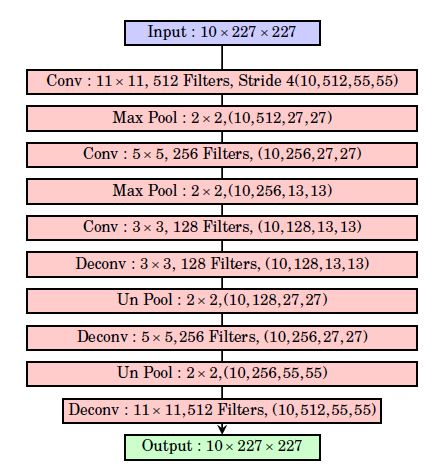
\includegraphics [scale=1]{images/STSAE.JPG}
\centering
\label{fig:STSAE}
\end{figure}


The L2 regularized loss function is minimized over frames from the training video.

\begin{equation}
    \mathscr { L } ( W ) = \frac { 1 } { 2 N } \sum _ { i } \left\| \mathbf { x } _ { i } - f _ { W } \left( \mathbf { x } _ { i } \right) \right\| _ { 2 } ^ { 2 } + \nu \| W \| _ { 2 } ^ { 2 }
\end{equation}
In the above equation, the tensor $x_i \in R^{r\times c\times p}$ is a cuboid with spatial dimensions $r$, $c$ are the spatial dimensions and p is the number of frames temporally back into the past, with hyper-parameter
$\nu$ which balances the reconstruction error and norm of the parameters, and $N$ is the mini-batch size.

%give refs
In the model discussed in \cite{Chong2017} is shown in the figure~\ref{fig:CLSTMAE}. The reconstruction error map at frame $t$ is given by $E _ { t } = \left| X _ { t } - \hat { X } _ { t } \right|$ while the temporal regularity score is given by the inverted, normalized reconstruction error :

\begin{equation}
    s ( t ) = 1 - \frac { \sum _ { ( x , y ) } E _ { t } - \min _ { ( x , y ) } \left( E _ { t } \right) } { \max _ { ( x , y ) } \left( E _ { t } \right) }
\end{equation}

In this equation, the $\sigma$ operators for min and max are directly across the spatial indices $x,y$. One could either directly use the reconstruction error as the anomaly score or use Mahalanobis distance. This is evaluated as the error between the original tensor and the reconstruction from the auto-encoder.

\begin{figure}[H]
\caption{Convolutional LSTM based autoencoder}
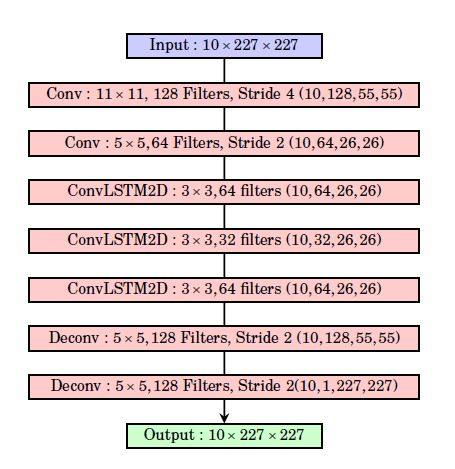
\includegraphics [scale=1]{images/ConvLSTMAE.JPG}
\centering
\label{fig:CLSTMAE}
\end{figure}

\subsubsection{Sparse Autoencoders}
Sparse autoencoders are acting in a similar way as the normal autoencoder, but it has higher number of hidden units than the number of input neurons. Using a structure like that we can still find some interesting patterns in image sequences and can be used for anomlay detection purposes. This generally involves a sparsity penalty $\Omega(h)$ on the latent layer in addition to the reconstruction error.

\begin{equation}
    L(x, g(f(x))) + \Omega(h)
\end{equation}
Here $g(h)$ is the decoder input and $h = f(x)$ which is the decoder output.

In the research published by Medhini et. al. \cite{sparse} describes a system that uses local and global descriptors that can identify an localize anomalies in a video frame. The local descriptors aid in learning local and temporal relationships which is utilized for localizing anomalies and global descriptos constructed using deep sparse autoencoders are used for interpreting the video as a whole. 



\subsubsection{Contractive Autoencoders}

The contractive autoencoders add the jacobian of the latent space representation to the reconstruction loss and and due to that, the latent space representation does not vary for small changes in the input \cite{Rifai:2011:CAE:3104482.3104587}. If the latent space representation z is $z = f(x)$, and the decoder mapping back to the input image spcae, $r(x) = g(z)$. The regularized loss function can be written as,

\begin{equation}
    \mathscr { L } ( W ) = \mathbb { E } _ { \mathbf { X } \sim X _ { \text { train } } } \left[ L ( \mathbf { x } , r ( \mathbf { x } ) ) + \lambda \left\| \frac { \partial f ( \mathbf { x } ) } { \partial \mathbf { x } } \right\| \right]
\end{equation}

Due to the regularized error function, the autoencoder becomes less sensitive to the input variation. But enforcement of the minimal reconstruction error keeps it sensitive to the manifold having higher density. These type of autoencoders capture the variations along the manifold but not orthogonal to it, or in other words, it estimates the tangent plane of the data manifold. \cite{22}.

\subsubsection{De-Noising autoencoders}
These autoencoders are well known for being robust feature extraction methods in the domain of unsupervised learning \cite{41}. Instead of reconstruction error minimization, reconstruction from the corrupted inputs is used. Stacked De-Noising Autoencoders (SDAE) are used to learn representations from a video using both appearance and motion information. Appearance is captured using raw values and motion information is captured using the optical flow between consecutive frames\cite{42}. These two types of SDAE pipelines are coupled together to learn a joint representation that captures both the above aspects.


\subsubsection{Deep Belief Networks}

These type of networks are created by stacking multiple hidden layers. Restricted Boltzmann Machines \gls{rbm}s can be stacked and trained in a greedy manner to form so-called Deep Belief Networks (DBN). Those are trained in an unsupervised manner in a greedy fashion to perform feature learning. They can reconstruct the original inputs and thus called generative models. 

In \cite{44} the DBNs have been used to represent raw image value representations. 
They have presented a unified energy-based framework for video anomaly detection. Their  method is based on RBMs (DBNs) to capture data regularity. Their system can distinguish and localize the irregular events. It is trained directly on the image pixels in a completely unsupervised manner. For video streaming, they further introduce a streaming version of their method that can incrementally update the parameters when new video frames arrive.

\subsection{Predictive Modeling}

If the current output frame at time $t$  is $X_t$, the basic idea of predictive modeling is that to represent the current frame in terms of past p frames $[X_{t-1},X_{t-1},.....,X_{t-p-1},X_{t-p}]$. This principal is used in  auto-regressive models for time series analysis which employs a linear function over the past data. The same is used with non-linear functions such as sigmoid functions in Recurrent Neural Networks(\gls{rnn}), modeled as recurrent relationships. The standard method for these type of modeling is the \gls{lstm} which in fact is a extended \gls{rnn} that has a gating functionality introduced in order to cater for the issue of vanishing gradient that was present in normal \gls{rnn}s when they were subject to backpropagation through time.
Recently there have been some researches done on the video prediction domain using convolution networks by minimizing mean squared error between predicted and future frame \cite{6}. A similar research was performed in \cite{50} using a \gls{cnn}-LSTM-deConv network by combining mean sqared error and adverserial loss.

\subsubsection{Usages of \gls{lstm} (Long-Short-Term-Memory)}

LSTMs are capable of remembering past frames while resolving issues aroused by vanishing gradient. This is performed by enabling various gate mechanisms that allow it to filter and carry forward the required information and retain only the necessary part. \gls{lstm} principal is used combined with other models as well. One such successful combination is Convolutional \gls{lstm}, which is a \gls{lstm} network formed in a 2D convolution network pattern.   
\subsubsection{Convolutional \gls{lstm}}

Convolutional long short term memory (\gls{convlstm}) is an encoder model that is a composite of the \gls{lstm} model and the encoder decoder model. The fully connected \gls{lstm} is a powerful model but it contains too much redundancy for spatial data. Convolutional \gls{lstm} takes a encoding -forecasting structure that has stacks of Concolutional \gls{lstm} layers. 

This model is basically designed to overcome the major drawback of fully connected \gls{lstm} models. They have full connections of input-to-state and state-to-state transitions in which no spatial data is encoded. \gls{convlstm} is nothing but adding a convolution operator between state-to-state and input-to-state transitions. 
The key equations are for \gls{convlstm} are as below. The $*$ denotes the convolution operation and $\circ$ denotes the Hadamard product(the element-wise product of matrices).

\begin{equation}
    \begin{aligned} i _ { t } & = \sigma \left( W _ { x i } * \mathcal { X } _ { t } + W _ { h i } * \mathcal { H } _ { t - 1 } + W _ { c i } \circ \mathcal { C } _ { t - 1 } + b _ { i } \right) \\ f _ { t } & = \sigma \left( W _ { x f } * \mathcal { X } _ { t } + W _ { h f } * \mathcal { H } _ { t - 1 } + W _ { c f } \circ \mathcal { C } _ { t - 1 } + b _ { f } \right) \\ \mathcal { C } _ { t } & = f _ { t } \circ \mathcal { C } _ { t - 1 } + i _ { t } \circ \tanh \left( W _ { x c } * \mathcal { X } _ { t } + W _ { h c } * \mathcal { H } _ { t - 1 } + b _ { c } \right) \\ o _ { t } & = \sigma \left( W _ { x o } * \mathcal { X } _ { t } + W _ { h o } * \mathcal { H } _ { t - 1 } + W _ { c o } \circ \mathcal { C } _ { t } + b _ { o } \right) \\ \mathcal { H } _ { t } & = o _ { t } \circ \tanh \left( \mathcal { C } _ { t } \right) \end{aligned}
\end{equation}

Encoding network compresses the input tensor to the hidden state while the forecasting network unfolds the hidden state network to make the prediction. The hidden representations can be used to capture moving objects like in the research the main objective would be to capture moving pedestrians. If a larger kernel is used, faster moving objects can be captured and if a smaller kernel is used, slower objects can be captured \cite{51}.

An encoder decoder model is used in the researches performed in \cite{52} and \cite{53} with some outstanding results. In their models, a \gls{convlstm} model was used as a unit in a composite \gls{lstm} model following an encoder decoder model, with two branches, one for reconstruction and the other for prediction. 


\subsubsection{Slow Feature Analysis (\gls{sfa})}
Slow feature analysis is based on the principal of slow features. In a series of image frames that change over time, or in other words, in a video frame, there are slowly moving features that can be captured. Even though the individual pixel values change drastically, and more frequently over time, these slow features are not changing as  frequent as much as in each pixels. These higher order internal visual representations very slow on time scale and identifying these would be useful in prediction of the future inputs and thus formulating a anomaly detection framework. This is entirely based on the slowness principal. 

The Slow Feature Analysis algorithm formalizes the general intuition behind the slowness principle as a non-linear optimization problem : Given a (potentially high-dimensional) input signal $x(t)$ , find functions $g_j(x)$ such that the output signals. This is an optimization problem which is denoted by the following equations.

\begin{figure}[H]
\caption{SFA}
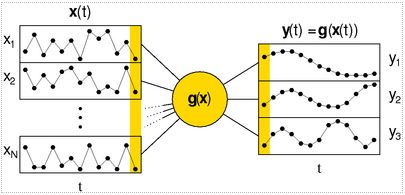
\includegraphics [scale=1]{images/SFA.JPG}
\centering
\label{fig:sfa}
\end{figure}


\begin{equation}
    y _ { j } ( t ) : = g _ { j } ( \mathbf { x } ( t ) )
\end{equation}

\emph{Optimization problem}
\begin{itemize}
    \item Minimize : $\Delta \left( y _ { j } \right) : = \left\langle \dot { y } _ { j } ^ { 2 } \right\rangle _ { t }$
\end{itemize}


\emph{Constraints:}
\begin{itemize}
    \item Zero mean : $\left\langle y _ { j } \right\rangle _ { t } = 0$
    \item Unit variance : $\left\langle y _ { j } ^ { 2 } \right\rangle _ { t } = 1$
    \item De-correlation of different signal outputs : $\forall i < j : \left\langle y _ { i } y _ { j } \right\rangle _ { t } = 0$
\end{itemize}


The constraints enforce the representation to have a unique solution and unit covariance to avoid trivial zero solution. Also uses feature de-correlation to avoid redundancy in features.

In \cite{58} and \cite{59} \gls{sfa} has been used for pattern recognition. An incremental updating mechanism of slow features was introduced by the authours in \cite{60}. The \gls{sfa} here is calculated using the batch \gls{pca} method by iterating twice.The first iteration is applied to whiten the inputs and the second one is applied on the derivative of
the normalized input to evaluate the flow features. In order to produce a traceable solution, another two layer localized \gls{sfa} architecture is introduced by the authors of \cite{61} 

\subsubsection{Other Predictive Models}

2D convolution nets are appropriate for image recognition and detection tasks, but they are not a good fit in terms of detecting the temporal information encoded in consecutive frames in video analysis tasks. As a solution, the authors in \cite{20} are using a 3D convolutional architecture, which is used in the form of an autoencoder. Such an autoencoder is capable of learning features that are invariant to spatio-temporal changes or in other words, movement, encoded by the 3D convolutional feature maps. The kernel is a 3d tensor and the output of such a kernel is a 3D tensor with one temporal dimension and are expected to summarize motion information. Authors in \cite{55} have proposed to use 3D kernel by stacking T-frames together, as in \cite{34}.

Another prediction model is used in \cite{62} in which a convolutional feature representation was fed into \gls{lstm} model to predict the latent representation. and the prediction error was used to evaluate anomalies in a robotics application. In \cite{63} authors have attempted to create a video forgery detection system by using a recurrent autoencoder that utilizes an \gls{lstm} which is used to model the temporal dependency between patches from a sequence of video frames. 



\subsection{Deep Generative Models}

If a supervised learning setup $\left( X _ { i } , y _ { i } \right) \in \mathbb { R } ^ { d } \times \left\{ C _ { j } \right\} _ { j = 1 } ^ { K }$ is indexed by $i$ where $i = 1:N$ in the data set, a generative model estimates the class conditional posterior distribution $P(X|y)$. This could become difficult if the input data is high dimensional images or spatio-temporal tensors. 

\subsubsection{Variational Autoencoders}

Variational Autoencoders basically models the data distribution $P(X)$ of a high dimensional input $X$ which could be an image or video. A encoder decoder architecture is used with some parameters $\theta$ and $\phi$ which essentially achieves the variational approximation of the  latent space. 

The goal of a variational autoencoder is to learn a low dimensional representation z by modeling P(X|z) with a simpler distribution, a Gaussian, i.e. $P ( X | z ; \theta ) = \mathscr { N } ( X | f ( z ; \theta ) , \sigma ^ { 2 } * I )$. The loss function has two terms. One is the reconstruction error and the other is the KL-divergence term between the latent space vector and the representation with a mean and standard deviation vector. 
Anomaly detection using variational autoencoders is experimented in \cite{64}. They evaluate the reconstruction probability $\mathbb { E } _ { q _ { \phi } ( \mathbf { z } | \mathbf { x } ) } \left[ \log p _ { \theta } ( \mathbf { x } | \mathbf { z } ) \right]$. 
First, for a new sample $x^{(i)}$ the mean and the standard deviation vectors are evaluated with the encoder, $(\mu_{z{(i)}}, \sigma_{z{(i)}}) = f_\theta(z|x^{(i)})$. Then the latent space vectors are sampled, $\boldsymbol { z } ^ { ( i , l ) } \sim \mathscr { N } \left( \boldsymbol { \mu } _ { \boldsymbol { z } ^ { ( i ) } } , \boldsymbol { \sigma } _ { \boldsymbol { z } ^ { ( i ) } } \right)$. Then the parameters for the input distribution are reconstructed using the $L$ samples, $\boldsymbol { \mu } _ { \hat { x } ^ { ( i , l ) } } , \boldsymbol { \sigma } _ { \hat { \mathbf { x } } ^ { ( i , l ) } } = g _ { \phi } ( \mathbf { x } | \mathbf { z } ^ { ( i , l ) } )$. Thus the reconstruction probability for the sample $x^(i)$ is given as follows.

\begin{equation}
P _ { \text { recon } } \left( \mathbf { x } ^ { ( i ) } \right) = \frac { 1 } { L } \sum _ { l = 1 } ^ { L } p _ { \theta } \left( \mathbf { x } ^ { ( i ) } | \boldsymbol { \mu } _ { \hat { \mathbf { x } } ^ { ( i , l ) } } , \boldsymbol { \sigma } _ { \hat { \mathbf { x } } ^ { ( i , l ) } } \right)
\end{equation}

In a variational autoencoder one of the main distinctions from a standard autoencoder is that, multiple samples drawn from the latent variable distribution lets the variability to be taken into account by the reconstruction error rather than in a case where latent variables are defined by deterministic mappings.

\subsubsection{Generative Adversarial Network(\gls{gan})}

\gls{gan}s were initially introduced by researches in \cite{65}. The \gls{gan} contains a generator G  which is a decoder usually and a discriminator which is usually a encoder. The task of the generator is to learn a distribution $p_g$ over the data $x$ via a mapping $G(Z)$ of the samples $z$ to 2D images in the image space manifold $X$, which is populated by normal samples. Here, $z$ is a 1D vector from the uniformly distributed input noise sampled from the latent space $Z$. The architecture of the generator G is a convolutional decoder architecture that utilizes a stack of strided convolutions. The discriminator D is a standard \gls{cnn} that maps 2D vectors to single scalar value. The generator output can be interpreted as probability (a value between 0 and 1) that indicates whether the given input is a real image sampled from $X$ or a generated image using G(z) by the generator G.

Discriminator D and Generator G are both simultaneously optimized through the minimax function mentioned below. 

\begin{equation}
    \min _ { G } \max _ { D } V ( D , G ) = \mathbb { E } _ { \mathbf { X } \sim p _ { \text { data } } } [ \log D ( \mathbf { x } ) ] + \mathbb { E } _ { \mathbf { z } \sim p _ { z } ( \mathbf { z } ) } [ \log ( 1 - D ( G ( \mathbf { z } ) ) ) ]
\end{equation}

The discriminator is optimized to give the maximum probability for "real" for those samples that are sampled from the real samples and "fake" to the samples that are generated by the generator. The main objective of the generator G is to minimize $\log ( 1 - D ( G ( \mathbf { z } ) ) )$ by maximizing $D ( G ( \mathbf { z } ) ) $, thus it essentially tries to fool the discriminator D by doing so. 

In \cite{67} a \gls{gan} model was applied for the task of identifying the anomalies in medical images. \gls{gan}s are generative models that are capable of generating training data points $\mathbf { x } \sim P _ { \mathrm { data } } ( \mathbf { x } )$  where $P _ { \mathrm { data } }$ represents the probability density of the training data points. For anomaly detection the basic idea is that while training, evaluation of normal vectors in the training set that has no anomalies. But in test negative log likelihood score is evaluated as the final anomaly score. \gls{gan}s provide a generative model without the definition of any parametric model.The generative model essentially minimizes the distance between training data distribution and the generative model. Since it does not use any parametric model, it is called an implicit generative model.  

In order to evaluate a likelihood for \gls{gan}s one requires a mapping from the image domain to the latent domain. This mapping is achieved by the authors in \cite{67}. In this research, the authors attempts to find a point $z$ in the latent space that corresponds to an image $G(z)$, which is more similar to the image x and this is located in manifold $X$. The similarity  of $x$ and $G(z)$  depends on how much the query image follows the data distribution $p_g$ which was used for training of the generator. 






\chapter{Methodology}
\newpage

In this research it is essential to explore all possible approaches for anomaly detection in video streams. The current literature in the domain directed the search towards deep learning as deep learning has become the new star in the area of video processing. The non-deep learning methods were very useful till the time that processing power was still an issue. But since processing power is available at a lower cost than before, it is always worth putting efforts in deep learning. On the other hand, deep learning is giving promising results that were not achievable through non-deep learning methods. In terms of accuracy and robustness deep learning proves to be the best. The only drawback is that it needs a huge amount of data to gain such better accuracy. Data is at abundance and with the huge amount of data at hand, a large processing power is also a requirement. Even though processing power is cheaper than before, it is still a considerable cost. If the target architecture is a deep learning based method, it should also be feasible in terms of cost of processing. Even though GPUs are available at a cheaper cost, the overall processing power depends on how much data that we are expecting to feed into our architecture, which may become expensive if the network is too complex. Also this system is a unsupervised system which is hard to achieve using the conventional non-deep learning based methods. Hence the only choice left is to use a deep learning method that can be trained without any supervision. 


\section{Proposed System}

The proposed system is a unsupervised (self-supervised) system that can be plugged into any environment and train on environment specific normality behavior and the system should be able to detect anomalies in a real time feed. This can be integrated to a mobile device and packaged so that it can be plugged to any cctv camera that captures the feed in real time. The anomalous behavior would be detected in frame level. The system can be extended to synthesize the local pixel level area that contained the anomaly. A flag will be inserted into a database and later the frame that contained anomalous behaviour could be reviewed. This system can be extended to classify the anomalies as a future project.





\section{Proposed Approach}

In chapter 2 (Literature Review), the deep learning based methods were discussed based on three main categories. Those categories are reconstruction based, spatio-temporal predictive models and generative models. The three categories can be summarized as below. Reconstruction based methods are focused on minimizing the reconstruction error of the representations built compared with the training samples from the normal distribution. In spatio-temporal predictive models, the videos are viewed as a spatio-temporal time series and  trained to minimize the prediction error on spatio-temporal sequences from the training series, where the length of the time window is a parameter. The generative models basically learn to generate models from the training distribution while minimizing the reconstruction error as well as distance between generated and training distribution. 

In the deep learning methods mentioned in the chapter 2, reconstruction models can be utilized for anomaly detection purposes but those models have one drawback that is not suitable for video anomaly detection tasks. Since the video analysis has a spatial dimension to be analyzed, certainly a convolutional model is required. But it also has a temporal dimension as well, thus, if we consider only the spatial dimension, the reconstruction will not be accurate as the temporal dimension is also containing some valuable feature information. Spatio-temporal auto-encoders and Convolutional \gls{lstm} learn a reconstruction based spatio-temporal predictive model that both use some form of  spatio-temporal regularity assumptions. Thus between mere predictive models and spatio temporal models, the requirement is more severed by the spatio temporal models that have some convolutional capabilities. Thus the Convolutional-LSTM suits the best.

As mentioned in the problem definition and the objective, the target system is a unsupervised system that can learn regardless of the environment present. The term 'unsupervised' can be interpreted as self-supervised in many of these algorithms as the training images that belong to normal class provide a degree of supervision implicitly even though there is no manual labeling involved. 
Since the type of normal behavior can be of a range that can vary, it is not possible to discreetly allocate classes to it. Thus having some variability introduced would help correctly identify the normal behavior and distinguish the abnormal behavior. For this purpose, variational autoencoders (\gls{vae}) are of great use. \gls{gan}s provide high quality reconstructions than \gls{vae}s but \gls{gan}s are hard to train. Usually a well trained generator of a \gls{gan} is able to generate samples that are from the same distribution as the training set and those images would be difficult to distinguish and theoretically a well trained discriminator would assign a probability value around 0.5 for those which are hardly distinguishable. But that discriminator would easily distinguish the samples that are outside the training distribution. If this discriminator is incorporated into a anomaly detection task, we can remove the generator and let the discriminator act alone as the sole jurisdiction of detecting anomalies. 

In \cite{54}, a convolutional representation of the input video is used as input to the convolutional \gls{lstm} and de-convolution is used to reconstruct the \gls{convlstm} output to the original resolution. The authors call this a \gls{convlstm} Autoencoder, though fundamentally it is not very different from a \gls{convlstm}. One drawback of this model was that they had to adjust thresholds each time it trains in a new environment in order to be able to distinguish the anomalies. Setting parameters appropriately is not an easy task for any average users who are not from a technical background. Hence the system should act as a black box to them that can plug and play. In a system that acts as a black box to the end user, there should not be any technical level adjustments to the system which requires some prior data science knowledge. In the current research, this drawback is going to be addressed with a alternative approach. Instead of manually setting threshold values, the idea is to let a discriminator of a trained \gls{gan} perform the judgment. The \gls{gan} and the \gls{convlstm} both need to be trained in the same environment and regardless of the input, the discriminator will be able to successfully distinguish the poorly reconstructed outputs from the \gls{convlstm} as anomalies. It is expected that since the reconstruction of an anomalous scene by \gls{convlstm} would be sufficiently deviated from the training distribution, the \gls{gan} discriminator is able to easily identify the presence of the anomaly, hence improved accuracy. The proposed system can be depicted as below.

\begin{figure}[H]
\caption{Methodology Summary}
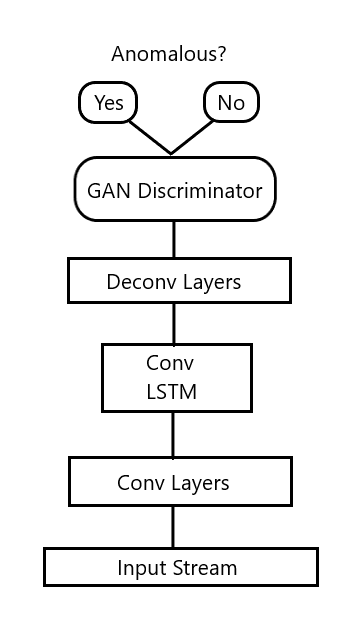
\includegraphics [scale=1]{images/method_1.png}
\centering
\label{fig:fig2}
\end{figure}




\newpage

\bibliographystyle{IEEEtran}
\bibliography{references}

\end{document}

